\subsection{Definition}
\begin{frame}
	\frametitle\insertsection
	\framesubtitle\empty
	\begin{center}
		\Large \textbf{\insertsubsection}
	\end{center}
\end{frame}
\begin{frame}
	\frametitle\insertsection
	\framesubtitle\insertsubsection
	\vspace{-2em}
	\begin{block}{Correlation}
		Process of determining which measurement could feasibly originate from a track.
	\end{block}
	\begin{figure}
		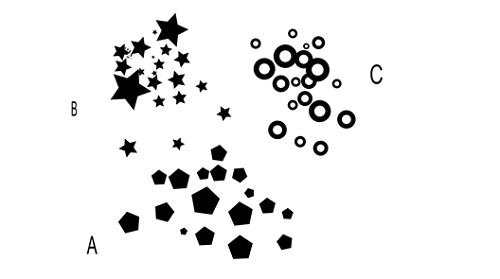
\includegraphics[scale=0.3333]{./img/data_correlation}
	\end{figure}
	\begin{itemize}
		\item {The correlation of a measurement to a track is statistically based, using the normalized statistical distance of the measurement from the track.}
	\end{itemize}
\end{frame}
\subsection{Correlation Process}
\begin{frame}
	\frametitle\insertsection
	\framesubtitle\empty
	\begin{center}
		\Large \textbf{\insertsubsection}
	\end{center}
\end{frame}
\begin{frame}
	\frametitle\insertsection
	\framesubtitle\insertsubsection
	\begin{figure}
		\caption{\textbf{Context of Data Correlation}}
		\scalebox{1}{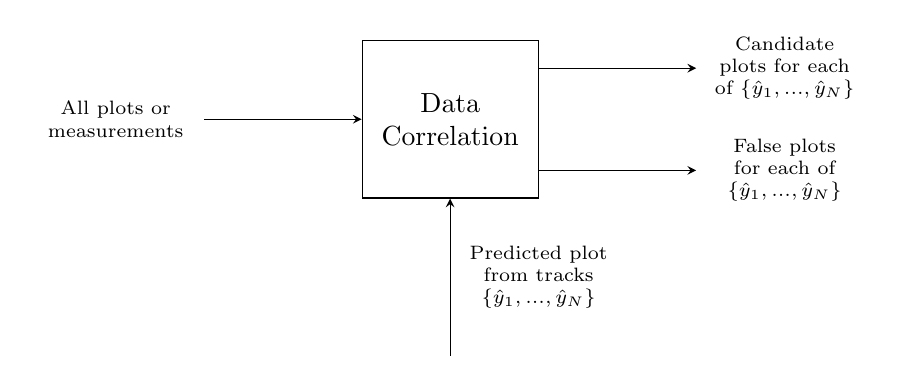
\begin{tikzpicture}[xscale=1,yscale=1,
	square/.style={rectangle, draw=black, text width=20mm, minimum height=20mm, align=center},
	label/.style={text width=20mm, align=center, font=\scriptsize},
	node distance= 2cm, >=stealth]
	
	%Nodes
	\node[square]	(dc)	at (0,0) {Data\\Correlation};
	
	%Lines
	\draw[black, <-] (dc.west) -- node [label, left, xshift=-10mm] {All plots or measurements} ++(-2,0);
	\draw[black, ->] (dc.30) -- node [label, right, xshift=10mm] {Candidate plots for each of $\{\hat{y}_1,...,\hat{y}_N\}$} ++(2,0);
	\draw[black, ->] (dc.330) -- node [label, right, xshift=10mm] {False plots for each of $\{\hat{y}_1,...,\hat{y}_N\}$} ++(2,0);
	\draw[black, <-] (dc.south) -- node [label, right] {Predicted plot from tracks $\{\hat{y}_1,...,\hat{y}_N\}$} ++(0,-2);
\end{tikzpicture}}
	\end{figure}
\end{frame}
\begin{frame}
	\frametitle\insertsection
	\framesubtitle\insertsubsection
	\vspace{-2em}
	\begin{itemize}
		\item {Gate are constructed around the predicted measurement for a track.}
		\begin{itemize}
			\item {If a measurement falls \textbf{inside} the gate, it becomes a candidate for association to the track.}
			\item {If a measurement falls \textbf{outside} the gate, it is not considered for association to the track.}
		\end{itemize}
		\item{Windows must take into account:}
		\begin{itemize}
			\item {Uncertainty in prediction.}
			\item {Uncertainty in new measurement.}
		\end{itemize}
	\end{itemize}
\end{frame}
\subsection{Gating Computation}
\begin{frame}
	\frametitle\insertsection
	\framesubtitle\empty
	\begin{center}
		\Large \textbf{\insertsubsection}
	\end{center}
\end{frame}
\begin{frame}
	\frametitle\insertsection
	\framesubtitle\insertsubsection
	\vspace{-2em}
	\begin{block}{Rectangular gating}
		\vspace{-1em}
		\begin{align*}
			|y_k-\hat{y}_{k|k-1}| \gtrless \kappa  \sigma_{k|k-1}
		\end{align*}
		where $\kappa$ is generally $ \geqslant$ 3
	\end{block}
	\begin{block}{Ellipsoidal gating}
		\vspace{-1em}
		\begin{align*}
		(y_{k} - \hat{y}_{k|k-1})^{T}S^{-1}_{k|k-1}(y_{k}-\hat{y}_{k|k-1}) \gtrless  \gamma_{G}
		\end{align*}
		where $\gamma_{G}$ is the gate threshold.
	\end{block}
\end{frame}
\begin{frame}
	\frametitle\insertsection
	\framesubtitle\insertsubsection
	\vspace{-2em}
	\begin{figure}
		\caption{\textbf{Illustration of Ellipsoidal gating}}
		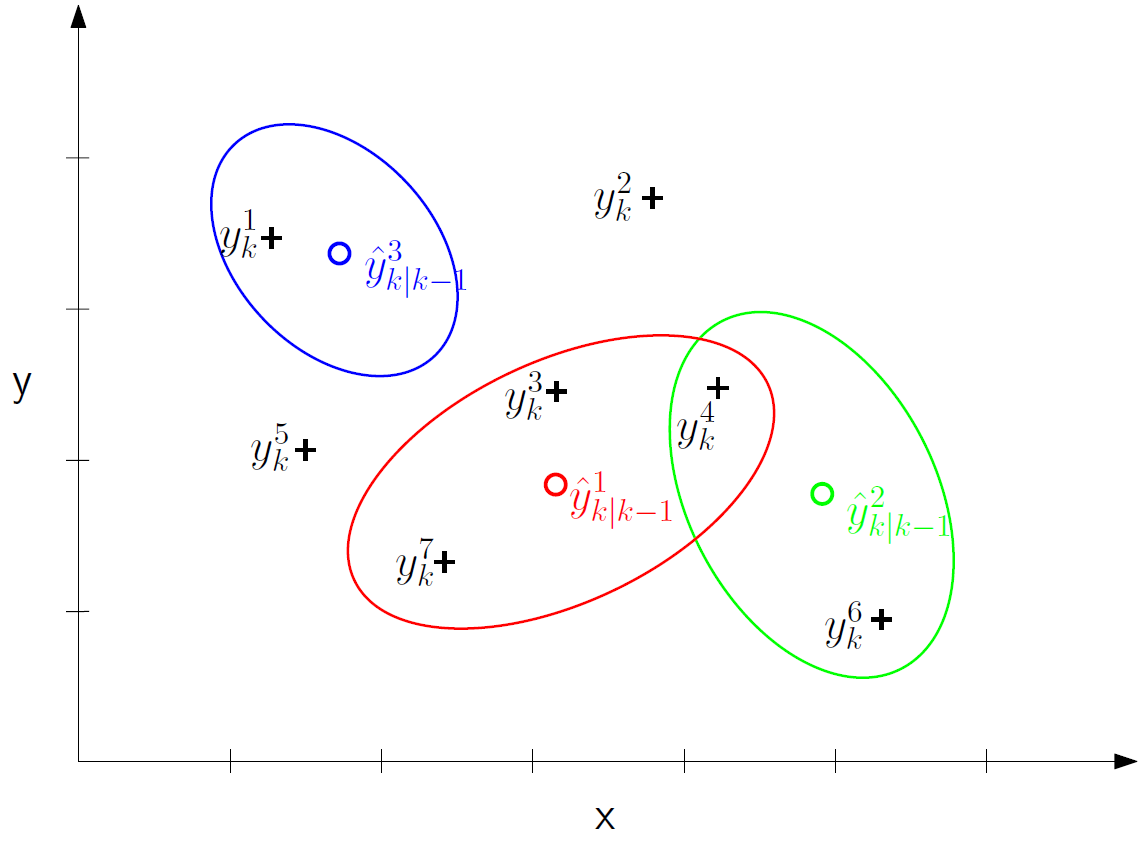
\includegraphics[scale=0.25]{./img/ellipsoidal}
	\end{figure}
	\vspace{-1em}
	$\hat{y}^i_{k|k-1}$ : Predicted measurement position for $i$th target\\
	$y^i_k$ \ \ \ \ \ : the $j$th measurement
\end{frame}
\begin{frame}
	\frametitle\insertsection
	\framesubtitle\insertsubsection
	\begin{block}{Ellipsoidal vs Rectangular Gating}
		\begin{itemize}
			\item {Rectangular gating is simpler to implement than ellipsoidal gating.}
			\item {Rectangular gating requires less computations than ellipsoidal gating.}
			\item {The ellipsoidal gate requires smaller area than the rectangular gate.}
		\end{itemize}
	\end{block}
\end{frame}